%%% Group 4: Tahoe, Ksenia Sokolova, Xinmeng Tong
%%% Computational Physics
%%% Spring, 2017

%%%%%%%%%%%%%%%%%%%%%%%%%%%%%%%%%%%%%%%%%%%%%%%%%%%%%%%%%%%%%%%%%%%%%%%%%%%%%%%%
%%% This code will develop a LaTeX'd writeup of the first group project
%%% assignment for PHYS566.
%%%%%%%%%%%%%%%%%%%%%%%%%%%%%%%%%%%%%%%%%%%%%%%%%%%%%%%%%%%%%%%%%%%%%%%%%%%%%%%%

% PACKAGES AND OTHER DOCUMENT CONFIGURATIONS
\documentclass[12pt]{article}
\usepackage[english]{babel}
\usepackage[utf8]{inputenc}
\usepackage{amsmath,amsfonts,amssymb}
\usepackage{graphicx,xcolor}
\usepackage{subfig}
\usepackage{booktabs}
\usepackage[left=2cm,%
right=2cm,%
top=2cm,%
bottom=2cm,%
headheight=11pt,%
letterpaper]{geometry}%
\usepackage{fancyhdr}
\pagestyle{fancy}
\lhead{\small\sffamily\bfseries\leftmark}%
\chead{}%
\rhead{\small\sffamily\bfseries\rightmark}
\renewcommand{\headrulewidth}{1pt}
\renewcommand{\footrulewidth}{1pt}
%\graphicspath{{}}

% Article Information
\title{Random Walks, the Diffusion Equation, and Cluster Growth}
\author{Tahoe Schrader, Ksenia Sokolova, Xinmeng Tong \\PHYS566}
\date{}

% Begin writing document
\begin{document}
\maketitle

% Start with the abstract

\abstract{In this assignment we study the random walks and their application in various systems. First we analyze the 2D random walk. Then observe that behavior of the random walkers can use to illustrated a diffusion process satisfying the diffusion equation, which is simulated using the finite difference form model. Furthermore, cluster growth is simulated by diffusion limited aggregation (DLA) model and the 'mass'-radius relation is given in our computation.
Our code is available on GitHub:

\url{https://github.com/tahoeschrader/PHYS566_group4_project-1a_walk-diffusion-cluster/tree/ksenia-presentation}}

\section{Theory}
\label{sec:theory}

\subsection{Random Walks in 2D}
Consider a 2D random walk. The displacement in the x direction is equal to the sum of displacement in x direction at every step. 

\begin{equation}
    X=\sum_{i=1}^{n} x_i
\end{equation}
The expectation value of displacement in the x direction can be found using the distributive property of the expectation for identically distributed random variables:
\begin{equation}
    <x>=\sum_{i=1}^{n} <x_i>=\sum_{i=1}^{n} (0.25)(-1)+(0.25)(1)=0
\end{equation}
This happens because there is equal probability to step right or left. The probability if 0.25 because overall we are in 2D, and so there is 50\% chance we will move in the vertical direction.

For the mean x-squared displacement we get
\begin{equation}
    <x^2>=<(x_1+x_2+x_3...)(x_1+x_2+x_3...)>
\end{equation}

\begin{equation}
    <x^2>=<x_1^2>+<x_2>^2+<x_3^2>+<x_1x_2>+<x_1x_3>+<x_2x_3>...
\end{equation}

We see that the result consist of combinations of $<x_i^2>$ and $<x_ix_j>$. Note that 
\begin{equation}
    E(x_ix_j)=1*0.25^2+1*0.25^2+(-1)*0.25^2+(-1)*0.25^2=0
\end{equation}

Therefore, all non-square terms vanish.

For the square terms, on the contrary, we always get $x_i=\pm 1$ and therefore $x_i^2=1$ and
\begin{equation}
    E(x_i^2)=1*0.25+1*0.25=0.5
\end{equation}

This means that 
\begin{equation}
    <x^2>=\sum_{i=1}^N <x_i^2>=\sum_{i=1}^N 0.5=0.5N
\end{equation}

Now, for the squared distance from the origin, we get
\begin{equation}
    <d^2>=<x^2+y^2>=<x^2>+<y^2>=0.5N+0.5N=N=4Dt
\end{equation}
if t=N, one step at one time interval.

Where we again used the distributivity of the mean and the fact that $E(x^2)=E(y^2)$ in case $P(x)=P(y)$


\subsection{Diffusion Equations and the Finite Difference Form}
\label{sec:diffusionequation}
The diffusion equation in $1D$ is written,
\begin{equation}
  \label{eq:diffusioneqn}
  \frac{\partial\rho(x,t)}{\partial t} = D\nabla^2\rho(x,t),
\end{equation}
where $D$ is the diffusion constant. Equation~\ref{eq:diffusioneqn} is turned into an iterable form by noting: $\rho(x,t) = \rho(i\Delta x, n\Delta t) = \rho(i,n)$. This is the finite difference form\footnote{The finite difference form must be used because the diffusion equation is time dependent. Therefore, a relaxation method cannot be used.}.

After using the formal definition of derivatives and algebraically manipulating Equation~\ref{eq:diffusioneqn} in the finite difference form, we get
\begin{equation}
  \label{eq:diffusioneqn-iterable}
  \rho(i,n+1) = \rho(i,n) + \frac{D\Delta t}{\Delta x^2}\left(\rho(i+1,n) + \rho(i-1,n) - 2\rho(i,n)\right),
\end{equation}
where $\Delta t$ and $\Delta x$ are the step sizes in an iteration. This solution requires knowledge of initial conditions. We must assume that the $x$ displacement is known at times prior to and including $t_n = n\Delta t$. Two consecutive steps prior to the first unknown step is sufficient to solve such an equation. Finally, to guarantee stability, the following criterion must be met
\begin{equation}
  \label{eq:stabilitycriterion}
  \Delta t \leq \frac{(\Delta x)^2}{2D}.
\end{equation}

We will use an initial density profile that is sharply peaked around $x=0$, but extends over a few grid sites to resemble a box. This is sufficient for generating the solution to the diffusion equation. Interestingly, after a couple iterations, the box profile will diffuse into a Gaussian normal distribution. The $1D$ Gaussian normal distribution has the form,
\begin{equation}
  \label{eq:gaussiandistribution}
  \rho(x,t) = \frac{1}{\sqrt{2\pi\sigma(t)^2}}\exp\left(-\frac{x^2}{2\sigma(t)^2}\right),
\end{equation}
where $\sigma(t) = \sqrt{2Dt}$.

The spatial expectation value, $\langle x(t)^2\rangle$, of Equation~\ref{eq:gaussiandistribution} is equal to $\sigma(t)^2$. Expectation values are calculated according to the equation
\begin{equation}
  \label{eq:expectationvalue}
  \langle x\rangle = \int_{-\infty}^\infty f(x)xdx,
\end{equation}
where $f(x)$ is the Guassian normal distribution for our purposes. Because we are looking for $\langle x^2\rangle$, Equation~\ref{eq:expectationvalue} becomes
\begin{align}
  \label{eq:spatialexpectationvalueintegral}
  \langle x^2\rangle &= \int_{-\infty}^\infty \frac{1}{\sqrt{2\pi\sigma(t)^2}}\exp\left(-\frac{x^2}{2\sigma(t)^2}\right) x^2 dx \notag \\
  &= 2\int_{0}^\infty \frac{1}{\sqrt{2\pi\sigma(t)^2}}\exp\left(-\frac{x^2}{2\sigma(t)^2}\right) x^2 dx.
\end{align}
The last step can be done because the $x^2$ term makes it an even function being symmetrically integrated about zero. Now, we make a change of variable $(x=\sigma\sqrt{2})$ to obtain, after a couple steps of algebra,
\begin{equation}
  \label{eq:spatialexpectationvalue-simplified}
  \langle x^2\rangle = \frac{4\sigma^2}{\sqrt{\pi}}\int_0^\infty x^2 \exp(-x^2)dx.
\end{equation}
Integrating the above equation by parts yields
\begin{equation}
  \label{eq:variancesolved}
  \langle x^2 \rangle = \sigma^2
\end{equation}
Typically, we call this equation the variance. % I used mathematica for the last step because actually integrating by parts was pretty difficult

\subsection{Cluster Growth with a DLA Model}
\label{sec:clusterDLAmodel}

The random walk idea could serve as a great tool to model cluster growth. One of the common cluster growth models is the diffusion limited aggregation (DLA) model, which starts with a seed particle at the origin of the system grid, and then release randomly generated starting walkers at a certain distance from the origin. The random walker is assumed to perform random walks until it reaches one of the boundary perimeter sites.  If so the sites that has been hit are updated to a new cluster. And the process is repeated until the cluster grows to a desired size. Compared to another model, Eden Model of cluster growth, the DLA cluster is sparser and has a crystal shape with many branches reaching out from the central cluster.

Analogue to a 2-D disk whose mass is $m(r)=\sigma \pi r^2$ with $\sigma$ being the mass per unit area, and a linear stick whose mass is $m(r)=\lambda r$ with $\lambda$ the linear mass density, a cluster has its the fractal or effective dimension which is defined to be $d_f$, where

\begin{equation}
  \label{eq:fractaldimension1}
     m(r)=C\cdot r^{d_f}
\end{equation}
thus
\begin{equation}
  \label{eq:fractaldimension2}
     log(m)=C+d_f\ log(r)
\end{equation}

For a cluster, assuming each walker is given a unit mass, then the mass $m$ is the number of walkers and $r$ is the radius of the cluster, with a proportionality constant $C$. If counting the particles within radius r around the origin seed position, we could find the relation:

\begin{equation}
  \label{eq:fractaldimension3}
     log(m) \sim d_f \cdot log(r)
\end{equation}
,which will be simulated using diffusion limited aggregation method later.


\section{Computations}
\label{sec:computations}

\subsection{Random Walks in 2D}
\label{sec:computationsRandomWalk}
To code the basic 2D walk, we assume that the probability to step in either direction left, right, up or down is the same. Then, for every step, we generate a random number. This is equivalent to drawing from Uniform (0,1). We assign every move to one of the segments of .25. If the random numbers falls within that value, we move in the assigned direction. The evidence for a successfully coded $2D$ walker program is given in Figure~\ref{fig:20steps} and \ref{fig:1000steps}.


\begin{figure}[!htb]
\minipage{0.5\textwidth}
  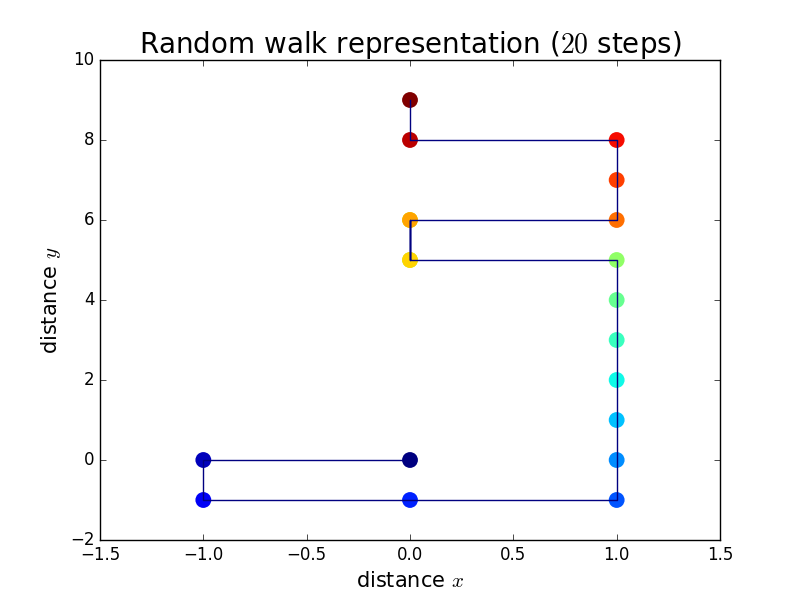
\includegraphics[width=\linewidth]{rWalk1.png}
  \caption{Random walk with 20 steps}\label{fig:20steps}
\endminipage\hfill
\minipage{0.5\textwidth}
  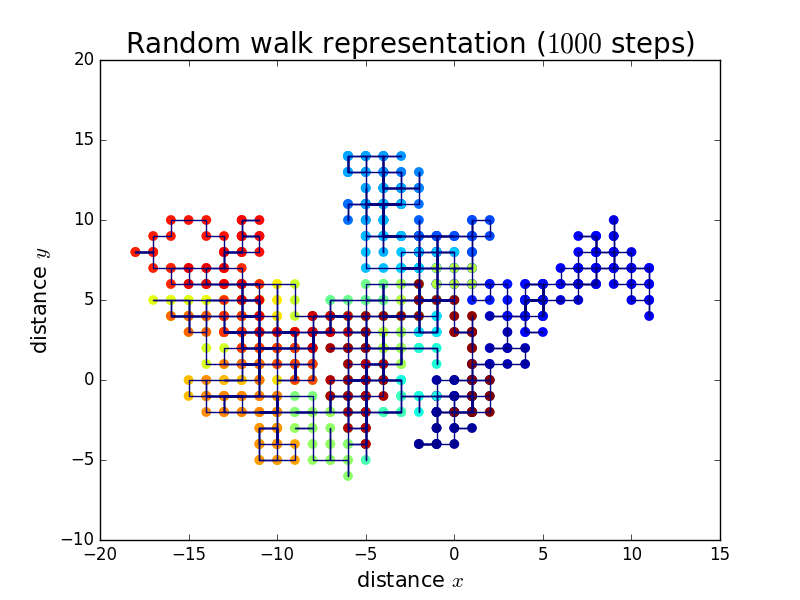
\includegraphics[width=\linewidth]{rWalk2.png}
  \caption{Random walk with 1000 steps}\label{fig:1000steps}
\endminipage\hfill
\end{figure}


Now, we can simulate $10^4$ random walks and compare the theoretical result of theory section with the simulations. 

First, we see that indeed $<x>\approx 0$, since the curve for $<x>$ oscillates around 0, as shown in Figure~\ref{fig:meanX}

We have also shown before that
\begin{equation}
    <x^2>=\sum_{i=1}^N <x_i^2>=\sum_{i=1}^N 0.5=0.5N
\end{equation}
When we simulate $<x^2>$ we indeed get the straight line with the slope equal to $0.5$ (see Figure~\ref{fig:meanX2}). 
The mean distance squared ($<d^2>$) graph also looks as expected, as a straight like with slope equal to 1 ((see Figure~\ref{fig:meanD2}).
Therefore, if $<d^2>=4Dt$, and steps are once at a time, diffusion constant is approximately $0.25$.

\begin{figure}[!htb]
\minipage{0.5\textwidth}
  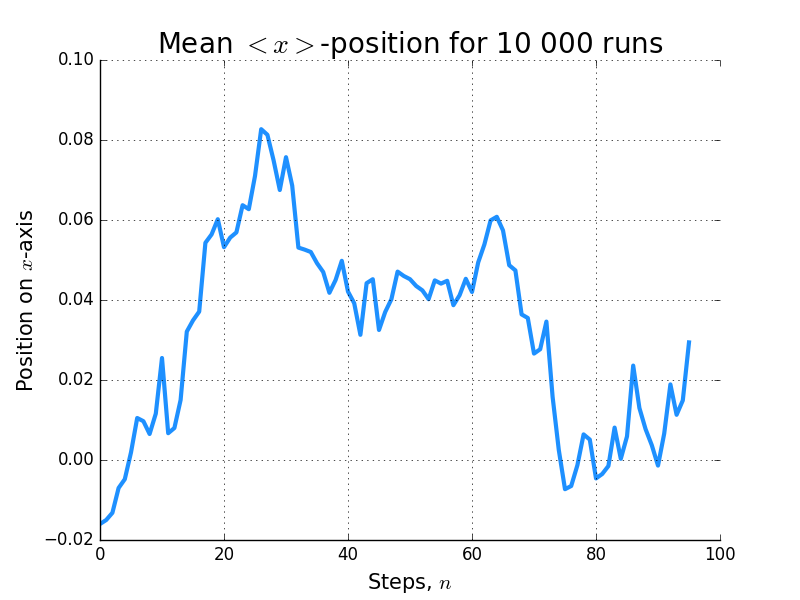
\includegraphics[width=\linewidth]{meanX.png}
  \caption{$<x>$ for random walk, $100$ steps}\label{fig:meanX}
\endminipage\hfill
\minipage{0.5\textwidth}
  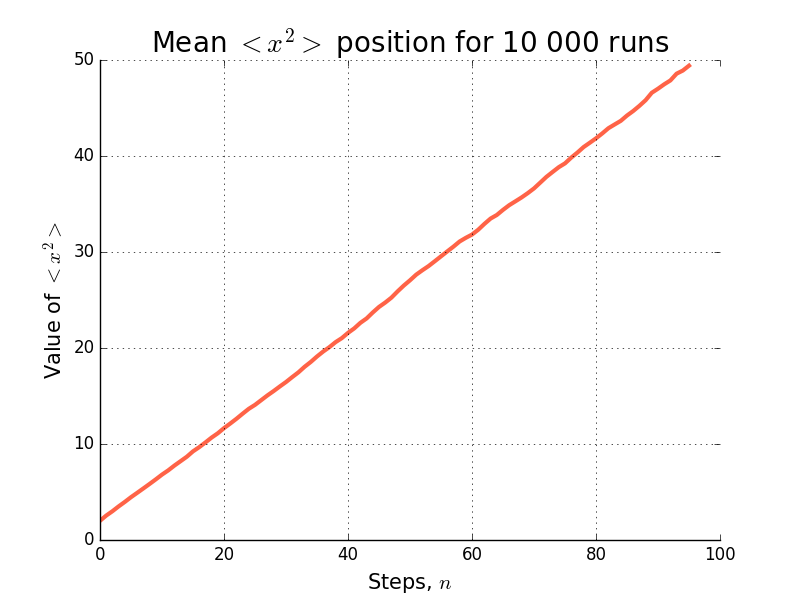
\includegraphics[width=\linewidth]{meanX2.png}
  \caption{$<x^2>$ for random walk, $100$ steps}\label{fig:meanX2}
\endminipage\hfill
\end{figure}
\begin{figure}[!htb]
\centerline{\minipage{0.5\textwidth}
  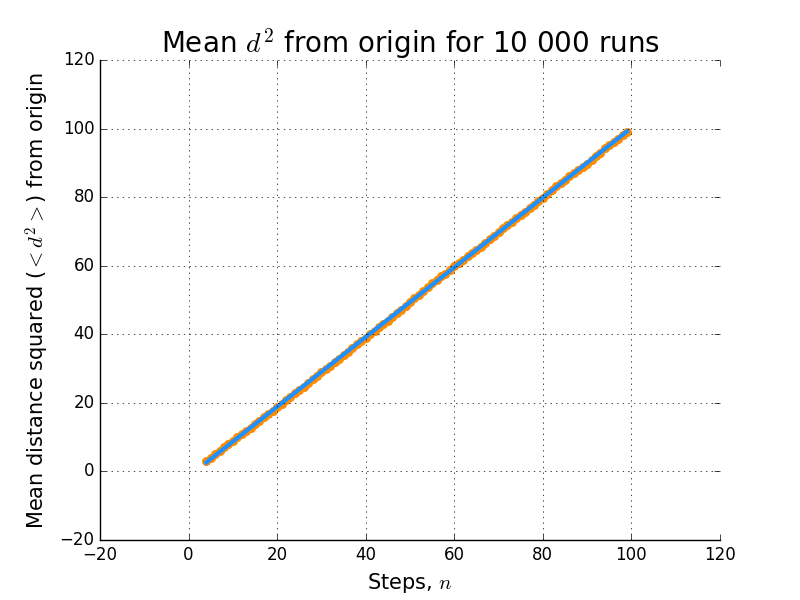
\includegraphics[width=\linewidth]{meanD2.png}
  \caption{$<d^2>$ for random walk, $100$ steps}\label{fig:meanD2}
  \endminipage}
\end{figure}

By observing the data, and noting that the $log(<d>)\,vs\,log(n)$ is linear, we can get a full form for $<d>$ as a function of $n$. 
\begin{equation}
    log(<d>)=log<a>+b log(n)
\end{equation}
\begin{equation}
    <d>=an^b
\end{equation}

 First, we plot $log(<d>)\,vs\,log(n)$, find a fit to the log curve and use the parameters to get the desired relation. In this case the curve was: 
\begin{equation}
    <d>=0.787n^{0.53}
\end{equation}
The power of $n$, which represents time in this case, is close to the expected $0.5$. The plots with fits can be seen on Figures~\ref{fig:meanDLog} and ~\ref{fig:meanD}.

\begin{figure}[!htb]
\minipage{0.5\textwidth}
  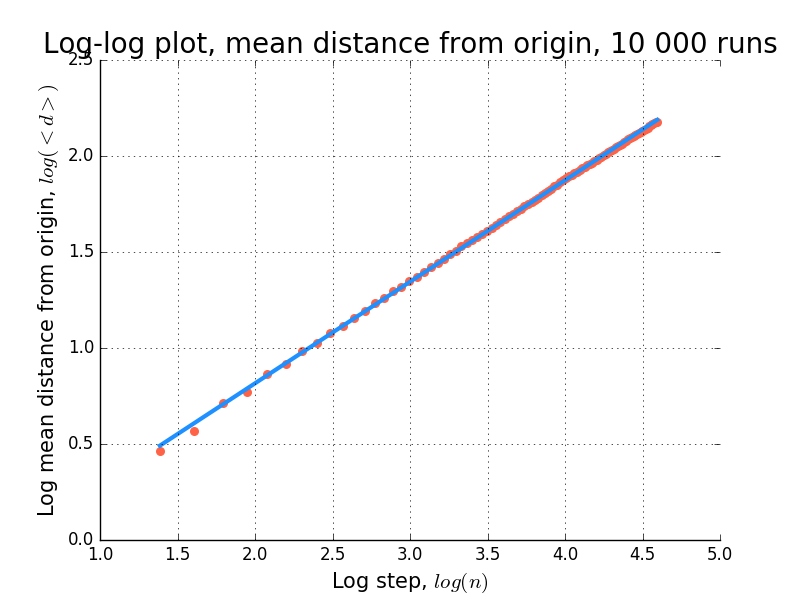
\includegraphics[width=\linewidth]{meanDLog.png}
  \caption{$log(<d>)\,vs\,log(n)$}\label{fig:meanDLog}
\endminipage\hfill
\minipage{0.5\textwidth}
  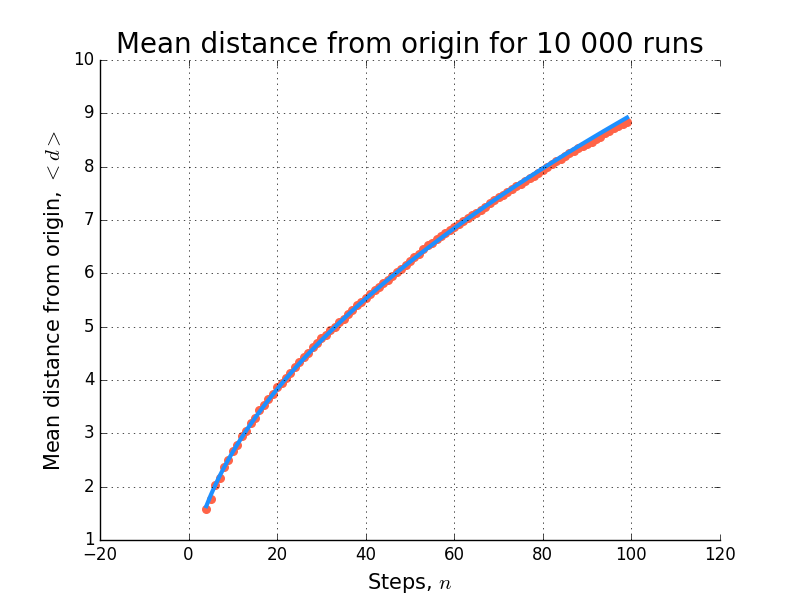
\includegraphics[width=\linewidth]{meanD.png}
  \caption{Graph for $<d>$ with a fit}\label{fig:meanD}
\endminipage\hfill
\end{figure}

An interesting addition to the random walk average in x direction would look at the graph (see Figure ~\ref{fig:randomMany}):
\begin{figure}[!htb]
\centerline{\minipage{0.5\textwidth}
  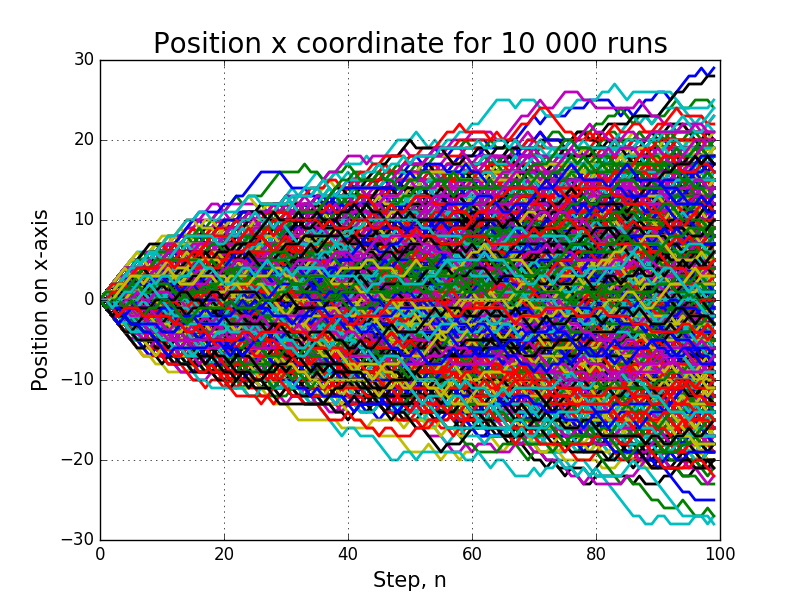
\includegraphics[width=\linewidth]{manyXpos.png}
  \caption{$x$ position for many runs of random walk}\label{fig:randomMany}
  \endminipage}
\end{figure}

\subsection{Diffusion of a Box Density Distribution}
\label{sec:diffusion-boxdensity}
Using the arguments in Section~\ref{sec:diffusionequation}, we solve the $1D$ Diffusion Equation over a period of time. Six different snapshots in time were then fit against Equation~\ref{eq:gaussiandistribution} to show a box shaped density will eventually diffuse into a Gaussian normal distribution.

It should be noted that it was important to place this box density far from the edges of the grid. Otherwise, the grid started to act as a makeshift boundary condition that, over time, made the distribution look less Gaussian. The initial distribution of our $1D$ diffusion solver is shown in Figure~\ref{fig:probdensityinit}.
\begin{figure}[!htb]
\centerline{\minipage{0.5\textwidth}
  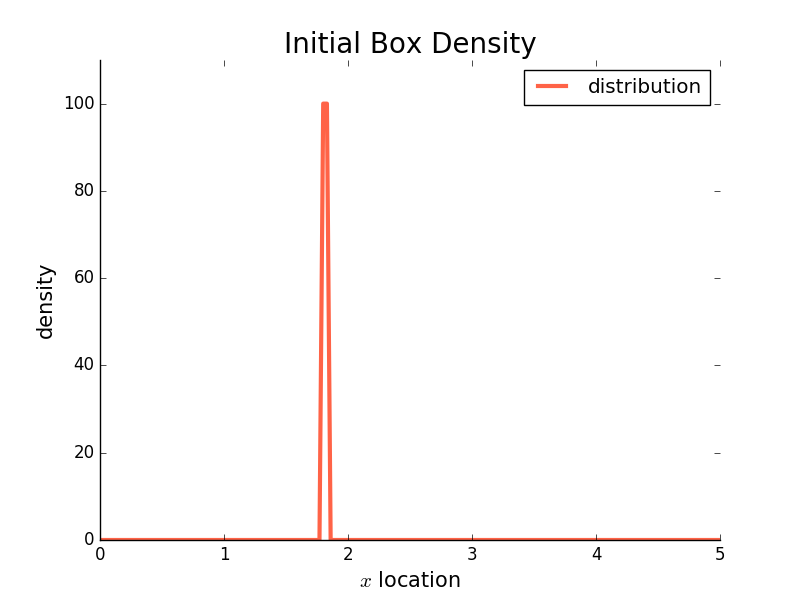
\includegraphics[width=\linewidth]{probdensityinit.png}
  \caption{initial box-shaped density}\label{fig:probdensityinit}
\endminipage}
\end{figure}

In Figures~\ref{fig:probdensity1}-\ref{fig:probdensity6}, we took snapshots of the $1D$ density equation and fit a Gaussian to the solution. A value of $\sigma$ was then extracted and compared to the analytical solution, $\sigma=\sqrt{2Dt}$. As can be seen, the fit worked exceptionally well for all time snapshots. The edge effects start to ruin our $\sigma$ fit in Figure~\ref{fig:probdensity6}.
\begin{figure}[!htb]
\minipage{0.5\textwidth}
  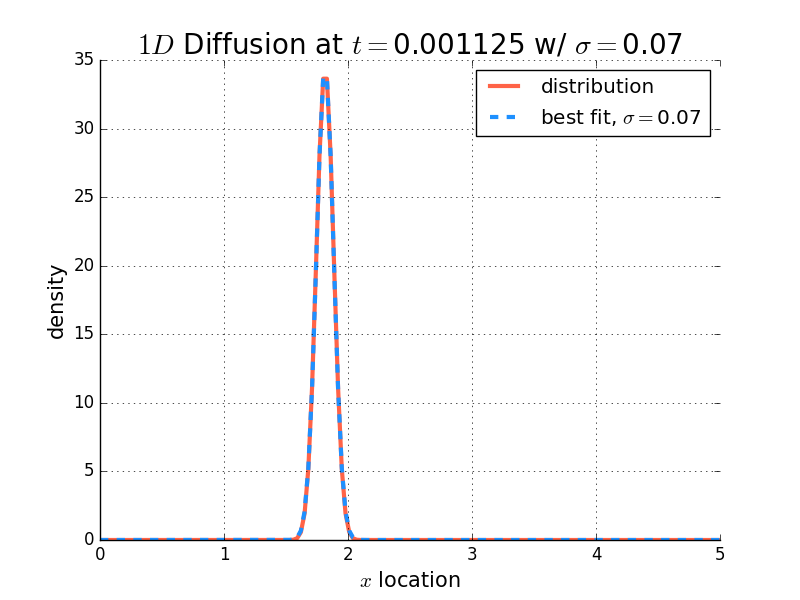
\includegraphics[width=\linewidth]{probdensityt10.png}
  \caption{}\label{fig:probdensity1}
\endminipage\hfill
\minipage{0.5\textwidth}
  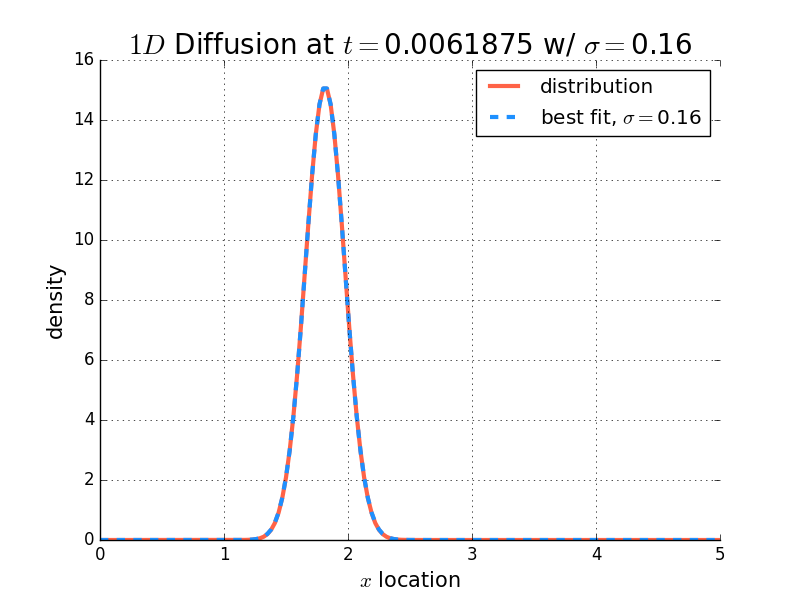
\includegraphics[width=\linewidth]{probdensityt55.png}
  \caption{}\label{fig:probdensity2}
\endminipage\hfill \\
\minipage{0.5\textwidth}
  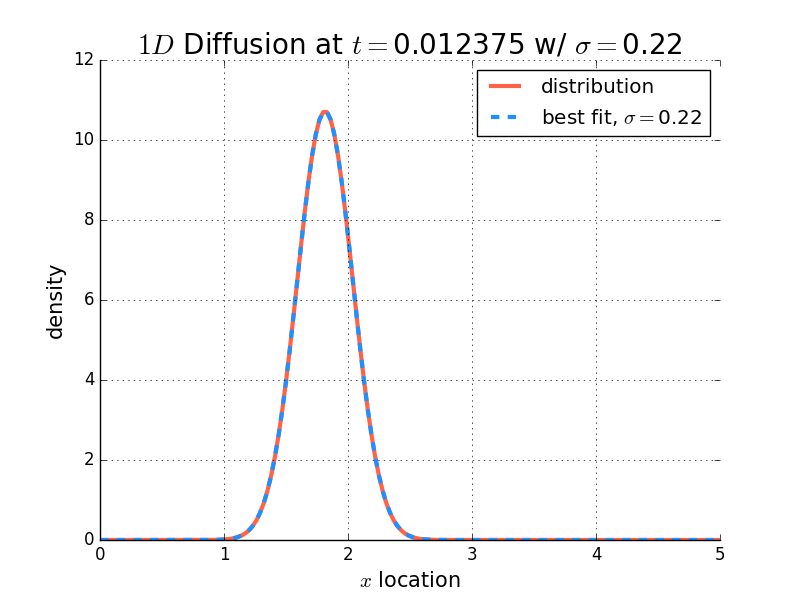
\includegraphics[width=\linewidth]{probdensityt110.png}
  \caption{}\label{fig:probdensity3}
\endminipage\hfill
\minipage{0.5\textwidth}
  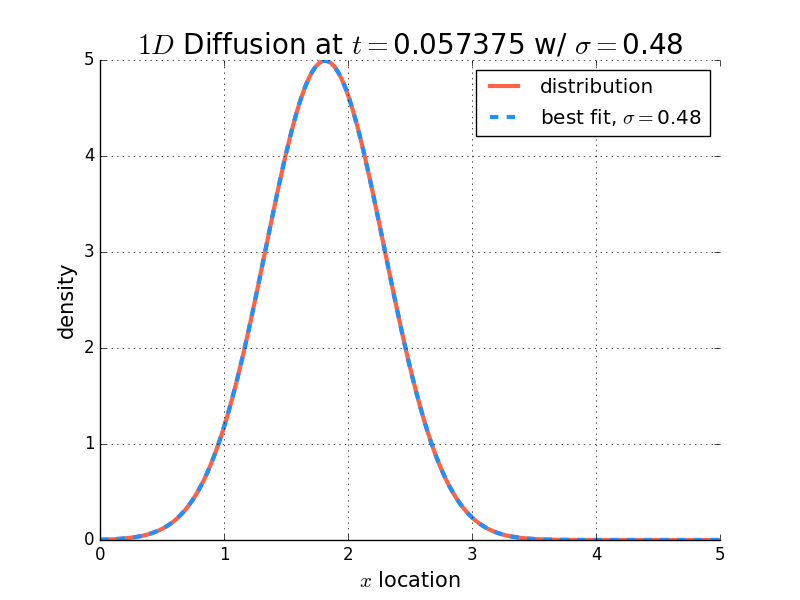
\includegraphics[width=\linewidth]{probdensityt510.png}
  \caption{}\label{fig:probdensity4}
\endminipage\hfill
\minipage{0.5\textwidth}
  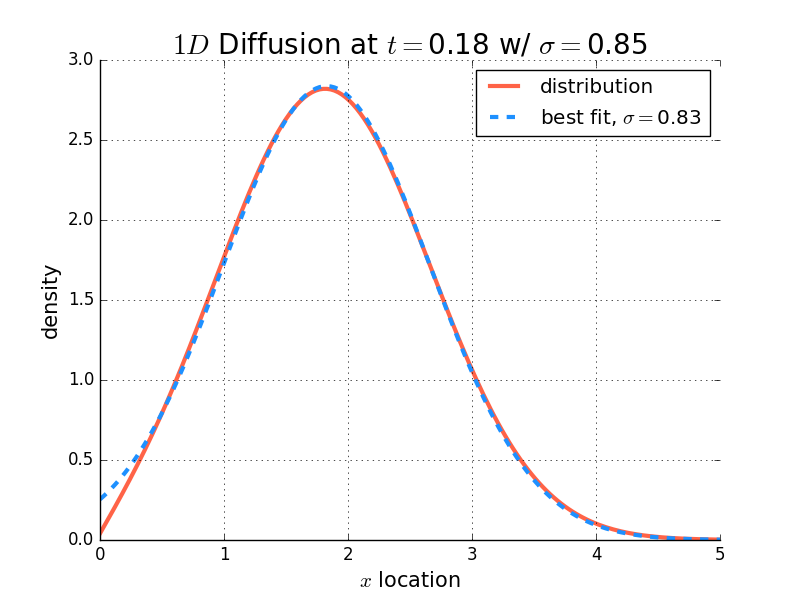
\includegraphics[width=\linewidth]{probdensityt1600.png}
  \caption{}\label{fig:probdensity5}
\endminipage\hfill
\minipage{0.5\textwidth}
  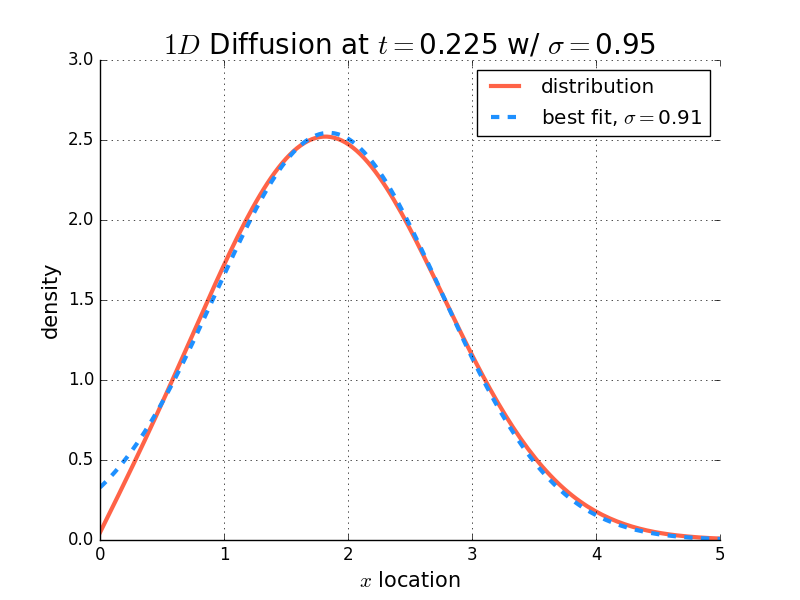
\includegraphics[width=\linewidth]{probdensityt2000.png}
  \caption{}\label{fig:probdensity6}
\endminipage\hfill
\end{figure}

\subsection{Growing Clusters and Extracting Fractal Dimensions}
\label{sec:clustersandfractals}

First, we simulate the DLA cluster by placing a seed in the middle. Then, the random walker is generated at the distance equal to the radius from the seed (center). This is done using a random number generator: we draw from (0,1) using random.random() and then multiply by $2\pi$ to get the angle in radians. Then we extract the coordinates in the matrix.

To enhance the speed of the code we use a matrix in the form (X, Y, label). Label corresponds to either out of bounds of radius (=2), occupied by walker (=1) or vacant (=0). 

Assumptions of our model: walker eventually finds either his 'friend', or in other words the other walker, or it wanders off to the edge of the square where it gets 'lost'. 

Please reference Figures ~\ref{fig:dla1} to ~\ref{fig:dla6} for the DLA structures for varying radius (12, 32, 52, 62, 72, 102 respectively).

\begin{figure}[!htb]
\minipage{0.4\textwidth}
  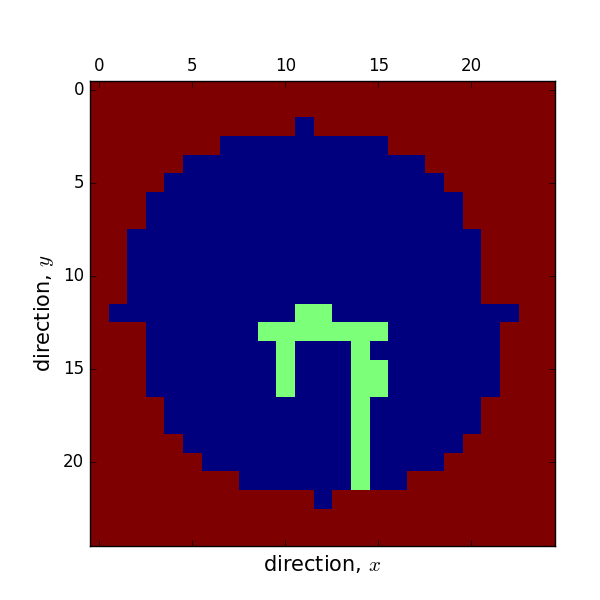
\includegraphics[width=\linewidth]{oneDLAcluster12run1.png}
  \caption{}\label{fig:dla1}
\endminipage\hfill
\minipage{0.4\textwidth}
  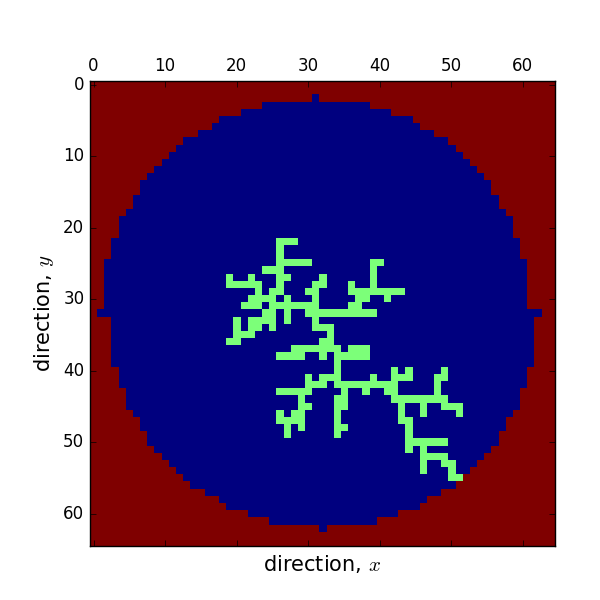
\includegraphics[width=\linewidth]{oneDLAcluster32run1.png}
  \caption{}\label{fig:dla2}
\endminipage\hfill \\
\minipage{0.4\textwidth}
  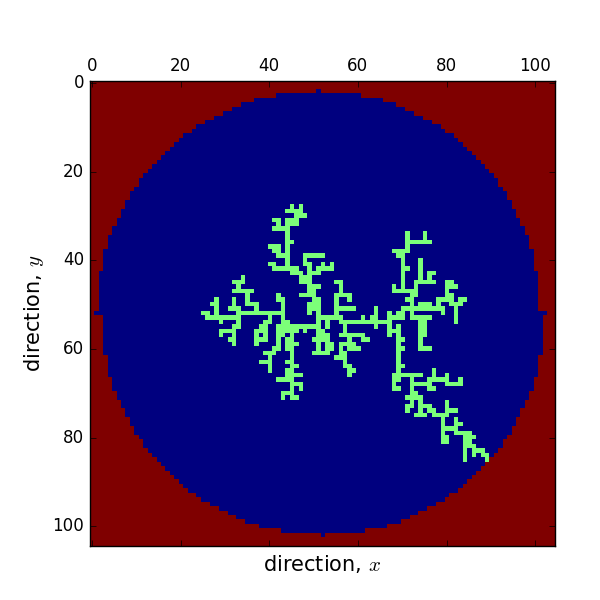
\includegraphics[width=\linewidth]{oneDLAcluster52run1.png}
  \caption{}\label{fig:dla3}
\endminipage\hfill
\minipage{0.4\textwidth}
  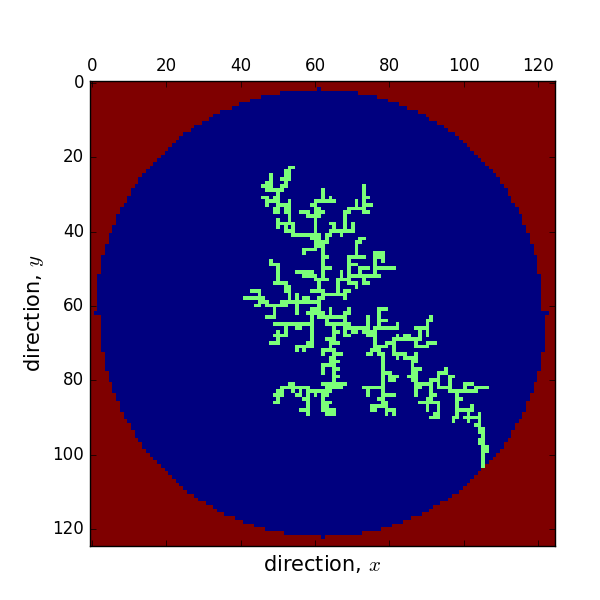
\includegraphics[width=\linewidth]{oneDLAcluster62run1.png}
  \caption{}\label{fig:dla4}
\endminipage\hfill
\minipage{0.4\textwidth}
  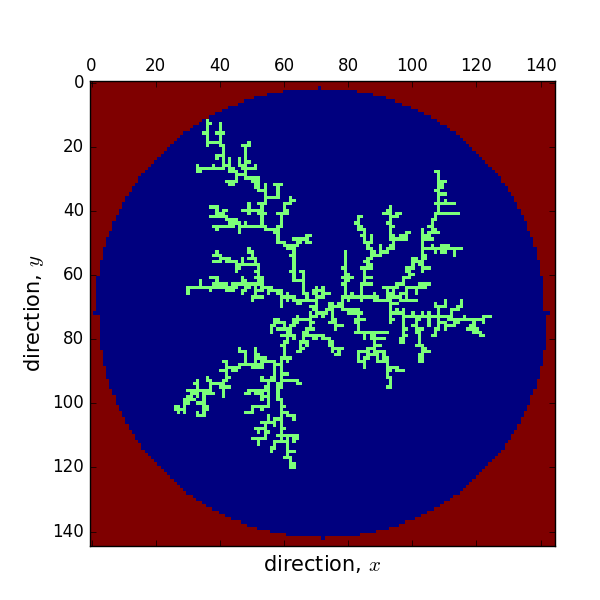
\includegraphics[width=\linewidth]{oneDLAcluster72run1.png}
  \caption{}\label{fig:dla5}
\endminipage\hfill
\minipage{0.4\textwidth}
  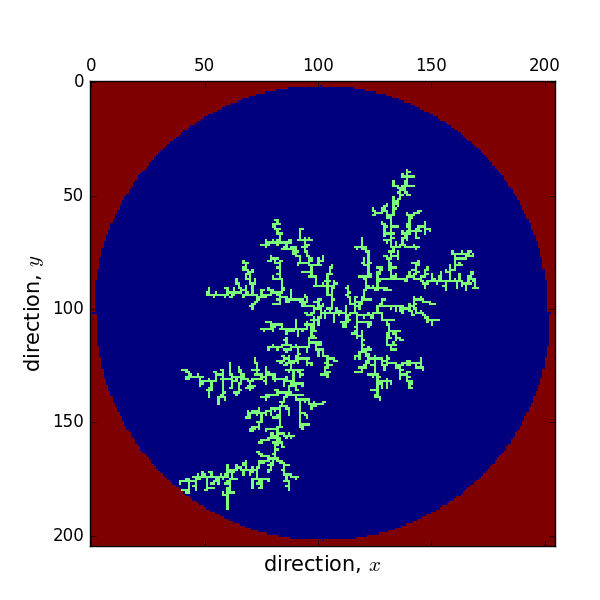
\includegraphics[width=\linewidth]{oneDLAcluster102radius.png}
  \caption{}\label{fig:dla6}
\endminipage\hfill
\end{figure}


By plotting the figure of $log(m)$ versus $log(r)$ simulated by the DLA cluster, the linear relation between these two parameters is obvious, with the slope of the straight line giving the fractal dimension of the generated cluster. And the proportionality constant is implied by the intercept of line with $y$ axis. We repeat the generation of cluster for 10 times to get the average fractal dimension with the given parameter so that the accuracy of $d_f$ is added. 

First, note that the trend line is very similar to the one in the textbook, and provides a good fit (Figure ~\ref{fig:fitDim}. 
The parameter of the slope shown is $2.06$

\begin{figure}[!htb]
\centerline{\minipage{0.5\textwidth}
  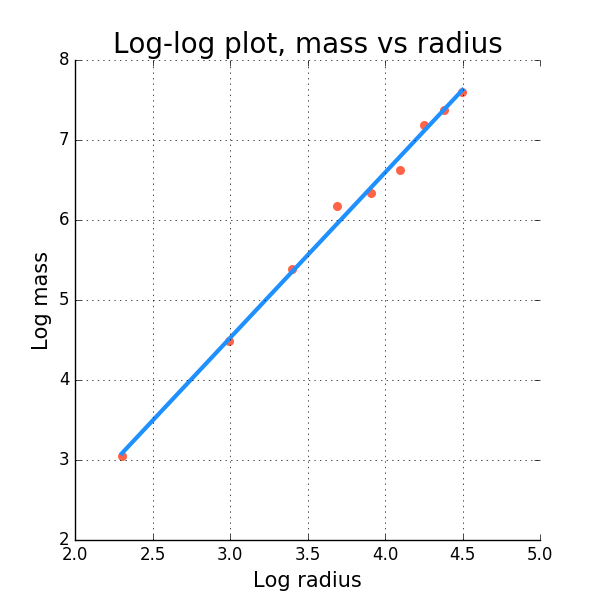
\includegraphics[width=\linewidth]{logRadiusMass1.png}
  \caption{Log radius vs log mass for the DLA cluster}\label{fig:fitDim}
  \endminipage}
\end{figure}

After 10 iterations, the resulting fractal dimensions were:

\textbf{2.067, 1.653, 1.877, 1.833, 1.607, 1.832,1.782, 1.712, 1.843, 1.862}

The mean value is then $1.807$. This is between 1 (line) and 2 (solid disc) and therefore close to the expected value for the dimensionality. 




\end{document}
